\section{HOPR incentivization mechanism}
HOPR incentivizes nodes in order to achieve correct transformation and delivery of mixnet packets.
This is accomplished using a mechanism called “Proof-Of-Relay” with the following layer 2 solutions which are both cost effective and privacy preserving.

\subsection{Probabilistic payments}
In traditional payment channels, two parties A and B lock some funds within a smart contract, make multiple transactions off-chain and only commit the aggregation on-chain.
\\~\\HOPR uses a concept called $acknowledgements$ which allows every node to creates a message that acknowledges the processing of the packet to the previous node. This acknowledgement contains the cryptographic material to unlock the payout for the previous node. Note that the acknowledgement is always sent to the previous node - even if there was no payment.
\\The fact that we are using payment channels implies that the last HOPR acknowledgement contains all previous incentives plus the incentive for the most recent interaction
$$value_(ACK_n) =\sum_{i=1}^nfee_{packet_i}$$ where $n$ is the total number of mixnet packets transformed.
\\~\\If B received $ACK_n$ before sending $packet_{n-1}$, it has no incentive to process $packet_{n-1}$ rather than $packet_{n-2}$.
\\~\\To avoid this limitation of traditional payment channels, HOPR utilizes probabilistic payments
\\~\\In probabilistic payments, the payouts use a concept called “tickets”, a ticket can be either a win or a loss with a certain winning probability. This means nodes are incentivized to continue relaying packets as they don’t know which ticket is a win.
\\~\\HOPR uses a custom-made layer 2 solution. It is inspired by payment channels and probabilistic payments where incentives can be claimed independently:
$$value ( ACK_i )=value ( ACK_j ) \quad for \quad i,j\in \{1,n\}$$
Hence, there is no added value in pretending packet loss or intentionally changing the order in which packets are processed.
\subsubsection{Channel management}
Initially, each payment channel in HOPR is \textit{closed} which means that in order to transfer packets, those channels have to be opened. Nodes can open channels to other nodes by either:
\begin{itemize}
    \item \textbf{Unidirectional channels:} Locking parts of their funds (staking) and calling the method \textit{open()}. This would allow them to act as a relayer and advertise their relay services without actually needing a confirmation from the other party.
    \item \textbf{Bidirectional channels:} Both parties agree on funding the channel in both directions. Node B can give their consent to node A for example to lock funds into the channel by signing an authorisation request sent by A $$auth(A: <\gamma>, B: <\delta>)$$ where $\gamma$ is the amount to be staked by A and $\delta$ is the amount to be staked by B. Both values can also be equal. 
    \\ A can then open the channel by calling the method \textit{openwithSignature()}. Once the call has succeeded, an on-chain event \textit{ChannelOpened} is thrown. The channel is now \textit{open}.
\end{itemize} 
As long as the channel remains open, nodes can claim their incentives for forwarding packets which is represented as tickets (see ticket section). Tickets are redeemed by dispatching a \textit{redeemTickets()} call. The balance of the channel is then updated according to the balance defined in the ticket.
\\~\\Nodes can close a payment channel in order to access their funds. There are three possible ways to do so:
\begin{itemize}
    \item \textbf{Interactively:} This is done by dispatching an on-chain call to \textit{close()}. This changes the on-chain state to $closed_A$ and the other party B can give their consent to close the channel by calling \textit{agreeB()}. This will allow B to redeem their previously unredeemed tickets. 
    \item \textbf{Using a timeout:} A can initiate the process by calling \textit{initiateClosure()}. This changes the state to $pending\_timeout$. Other nodes will have now time to claim not yet claimed tickets. Once the timeout is done, any of the involved parties can call \textit{withdraw()}. This turns the channel state into \textit{closed}. 
    \item \textbf{Immediately witn a signature:} This can be done using a single call to \textit{closewithSignature()} by one of the parties after the other party gives their consent. 
\end{itemize}

\begin{figure}[H]
    \centering
    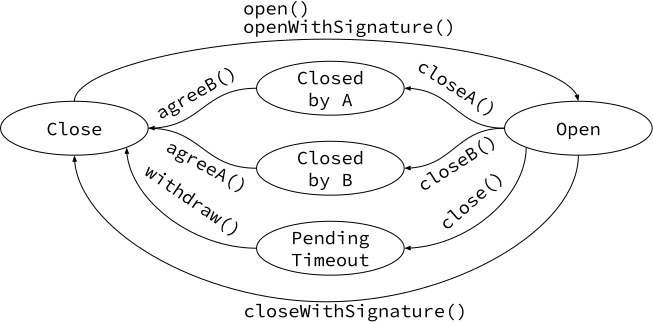
\includegraphics[width=\textwidth,keepaspectratio]{../yellowpaper/images/payment_channel_graph.png}
    \caption{Payment channel state graph}
    \label{fig:Payment channel graph}
\end{figure}
\subsection{On-chain Commitment}

\subsubsection*{Definition}
A commitment scheme is a protocol between usually two parties $A$ and $B$ and fulfills two properties (hiding and biding).
\\~\\\textbf{Hiding:} The ability to commit a value only known by the sender.
\\~\textbf{Binding:} The committed value must be the only one that the sender can compute and that validates during the reveal phase. 
\\~\\HOPR uses on-chain commitments to verify whether a ticket is a win or not in order to redeem it later on. The relayer doesn't know beforehand whether the ticket is a win or not until they receive an acknowledgment from the next downstream node eand can't change the outcome.
\subsubsection{Setup phase}
Once a node joins the HOPR network, it creates an iterated commitment and stores the opening key in the database. 
Iterated commitment scheme means $open_n$ opens $cm_n$ whereas $open_{n-1}$ opens $cm_{n-1}=open_n$ and so on. 
\newline The final commitment is computed as $cm_n:= h^n(r)$ where hash is a preimage-resistant hash function and 
$r$ is chosen uniformly at random by the node in order to prevent the issuer from knowing whether the ticket will be a win or not. 
\\~\\ Furthermore, it will prevent it from tweaking the given challenge such that the ticket cannot be a win.
The number of iterations $n$ can be chosen as a constant and should reflect the number of tickets a node intends to redeem.

\subsubsection{Opening phase}
In order to redeem a ticket, a node has to reveal the opening to the current commitment $cm_n$ that is stored in the smart contract. 
\\~The opening shouldn’t be revealed otherwise since it discloses whether a ticket is a win or not.
The ticket is a win if: $$h( t_h, r, open ) <P_w$$ where $$t_h:=h(t)$$
The opening is computed as $open_{n-1} = h^{n-1}(r)$ such that $cm_n=h( open_{n-1})$. 
\\~\\The on-chain logic verifies whether the latest opening $open_n$ indeed opens the current on-chain commitment $cm_n$. 
If this is the case, the current on-chain commitment is replaced by the given opening. 
\\~The on-chain keeps track of updates to the on-chain commitments to prevent double-spending. 
So whenever a node resets a commitment, a counter, namely $account.counter$ is increased and a call to $updateCommitment$ invalidates all previously unredeemed tickets.



\subsection{Proof Of Relay}

HOPR incentivizes packet transformation and delivery using a mechanism called “Proof-Of-Relay”.
This mechanism makes sure nodes relay services are verifiable.
\paragraph{Construction}
\begin{itemize}
    \item Every packet is sent together with a ticket.
    \item Each ticket contains a challenge.
    \item The validity of a ticket can only be checked on reception of the packet but the on-chain logic enforces a solution to the challenge stated in the ticket.
\end{itemize}

Since “Proof-Of-Relay” is used to make the relay services of nodes verifiable, it is the duty of each node to check that given challenges are derivable from the given and the expected information.
Packets with inappropriate challenges should be dropped as they might not lead to winning tickets.
Therefore, the sender of the packet also provides a hint of the expected value that a node is supposed to get from the next downstream node (as explained in the ticket section).

\begin{figure}[H]
\begin{center}
    \begin{tabular}{| m{2em} | m{15em} | m{2em} |}
        \hline
        $\alpha$ & $\beta$                   & $\gamma$ \\
                 & \begin{tabular}{| m{2em} | m{3em} | m{6em} |}
            \hline
            $Y_B$ & $hint_B$ & $challenge_{BC}$ \\
            \hline
            $Y_C$ & $hint_C$ & $random$         \\
            \hline
            $Y_D$ & $hint_D$ & $random$         \\
            \hline
            \multicolumn{3}{| l |}{End}         \\
            \hline
        \end{tabular} &          \\[3em]
        \hline
    \end{tabular}
\end{center}
\caption{SPHINX with PoR}
\label{fig:SPHINX with PoR}
\end{figure}
